\documentclass[../access.tex]{subfiles}
\graphicspath{{\subfix{../Images}}}

\begin{document}
    \label{centralized-analysis}
    \subsubsection{Introduction}
    E-voting systems under a centralised paradigm (typically a server-client architecture) concentrate all processing power into a unit or cluster of processing units. This implies that the security of the system depends directly on the resources allocated to it, namely memory, storage, processing power, etc. A user's trust in a system is directly dependent on the security of the system, which is formally divided into discrete implementation criteria. As mentioned in Section \ref{background}, there are multiple strategies and tools to increase system security, but for this study, we are only interested in the ones implemented through cryptographic tools. As such, these systems can be characterised by the set of security criteria used to establish trust in the system, as well as the cryptographic tools with which they achieve this goal.
    \par
    These criteria have long been proposed by researchers as a way to quantify and establish trust in the proposed system, albeit in an informal fashion. The importance of such elements is evident in all publications considered. As publications grew, a consensus began to take shape among the researchers dedicated to this area but lacking any formalization. As a consequence, it is common to see independent researchers referencing the same criterion but with different names and similar, but not identical, definitions of it. As such, the goal of this analysis is the identification and characterization of these criteria into a unified set.
    \par
    The implementation of these security features often relies on cryptographic methods that have been developed alongside these systems. Electronic voting systems are just one of the potential applications of the cryptographic methods developed from the ideas presented in \cite{Diffie1976}. The \textit{Diffie-Hellman Protocol} was the first implementation of such ideas \cite{Maurer2000}, which was soon followed by applications still used today such as Secure Shell (SSH), Transport Layer Security (TLS), Secure Sockets Layer (SSL), Public Key Infrastructure (PKI), Internet Key Exchange (IKE), and Internet Protocol Security (IPSec), among others less known \cite{Diffie1988}, \cite{Schneider1994} \cite{Ahmed2012}.

    \subsubsection{Classification Criteria for e-Voting Systems}
    \label{classification-criteria-centralized-systems}
    The majority of works presented use a classification framework to compare their solution with previous works. This type of analysis becomes more frequent as more e-voting systems are proposed through academic publications due to the enrichment of the set of previous works used for comparison.
    \par
    \cite{Neumann1993} in particular, presents one of the first attempts to formalise a "generic set of criteria in concept to existing security criteria" related to several other computer systems with strong security components. Publications prior to this one, such as \cite{Cohen1985}, \cite{Benaloh1986a}, and \cite{Fujioka1992}, used criteria to evaluate the solution proposed from a security standpoint, but only \cite{Neumann1993} did it explicitly and formally. As such, this publication has been referenced by later authors to introduce their own set of classification criteria.
    \par
    Though this logic may appear to have a common origin, in subsequent publications we were able to verify that the authors continue to diverge from a common set of listing criteria that varies highly in number and detail. Considering the lack of a common framework of analysis for these systems and the considerable size of the set of articles that we selected for analysis, we took the opportunity to execute a statistical analysis to determine the most common criteria considered among the pool of authors.
    \par
    We analysed the publications set, and we were able to extract two sets of security criteria standing on different levels of importance in the e-voting context. The first set was considered \textit{minimal} and contains the most common criteria found among them. The number of criteria considered varies significantly with authors, given the subjectivity associated with their choice. We also detected redundancy in larger criteria sets. The following statistical analysis defines each criterion considered so that it matches as closely as possible, starting from a base definition retrieved from the cited authors.
    \par
    The second set was found to be not as related to security itself, but perhaps more applicable as usability enhancers. These criteria, from here on considered \textit{additional}, can improve the experience of a voter with the system but do not increase the system's security, unlike the \textit{minimal} set, while still consuming significant resources.
    \par
    We follow these remarks with an enumeration and discrimination of the security criteria identified. This list also provides the answer to research question \textbf{RQA1}.

    \paragraph{Minimal Classification Criteria for Voting Systems}
    \label{minimum-classification-criteria}
    The following list contains a set of common criteria identified in the literature whose definitions were compiled from the individual explanations provided by the analysed works.
    \begin{enumerate}
        \item \textbf{Accuracy.} An accurate voting system does not allow changes to a vote after submission, changes to the final tally, or for invalid votes to be counted. Accurate voting systems also have the ability to detect and remove erroneous votes without invalidating the whole election. Accuracy can be quantified as the inverse of the overall probability of obtaining an erroneous final result \cite{Schneider2004}, \cite{Shamos1993}.
        
        \item \textbf{Eligibility.} A voting system implements eligibility if it allows \textit{only} registered or valid voters to submit votes. This also means that, in the final tally, only one vote per voter is counted \cite{Lee2000}.
        
        \item \textbf{Privacy.} If a voting system is able to remove all the links between the voter's personal information, which may be required for \textit{eligibility} purposes, and the vote submitted while preventing voters from disclosing what votes they cast, it is considered private. \cite{Hirt2000}, \cite{Benaloh1994}.
        
        \item \textbf{Verifiability.} Verifiable voting systems allow for independent confirmation of the final tally. This criterion is sometimes split into \textit{Individual} and \textit{Universal Verifiability} regarding the scope of the ability \cite{Rjaskova2002}, i.e., if individual votes can be verified or if it is limited to the final tally \cite{Sako1994}. Since the details that differentiate between these are outside the scope of this document, any system that supports any kind of verifiability is counted as such, regardless of its specific type.
        
        \item \textbf{Robustness.} Robust voting systems are able to prevent, or even withstand, dishonest voters, either individually or working in a coalition, in order to prevent the successful and correct completion of a voting exercise. Otherwise, they at least increase the probability of such an event being detected, either by design or by implementing consequences that make such act not profitable \cite{Schweisgut2006}.
    \end{enumerate}

    Table \ref{tab:e-voting-classification-criteria} summarises the grouping strategy used to deal with the high variability of denominations found in the publication set. It presents a summary of our findings in this regard, where publications are listed according to the exact denomination used to denote the criterion implemented. Due to the high degree of freedom each author used to name these properties and the limitations of space available, only the authors that mention the criterion under the considered name are listed, as well as the two most popular designations with the list of authors that used them. Definitions used by smaller groups of authors were simply indicated as such.
    \par
    In accordance with the majority of publications, these criteria are also referred to as \textit{security criteria}, given that the implementation of such features in an e-voting system directly translates into a more secure and reliable system.
    
    \begin{table*}[htbp]
        \footnotesize
        \begin{adjustwidth}{-1cm}{}
        \caption{Statistical analysis of the classification criteria}
            \begin{tabular}{@ {} p{1.0cm} p{5.0cm} p{3.0cm} p{2.0cm} m{3.5cm}  @{}}
                \hline
                \multicolumn{5}{c}{\textbf{Minimal Classification Criteria}} \\
                \hline
        %-------------------------------------------------------- ACCURACY ------------------------------------------------------------------------------------------------------
                \hline
                \multicolumn{1}{c|}{\multirow{7}{*}{\rotatebox[origin=c]{90}{Accuracy}}} & \multicolumn{3}{c|}{Referenced as:} & Also referenced as: \\
                \cline{2-5}
                \multicolumn{1}{c|}{} & \multicolumn{1}{c|}{"Accuracy" in:} & \multicolumn{1}{c|}{"Correctness" in:} & \multicolumn{1}{c|}{"Completeness" in:} & \multirow{6}{3.5cm}{Integrity (\cite{Ibrahim2003}, \cite{Chaieb2019}, \cite{Adiputra2019}, \cite{Chaieb2018}, \cite{Yang2020}), Data Integrity (\cite{Lee2017}), System Integrity (\cite{Neumann1993}), Tally Correctness (\cite{Juang1997}, \cite{Juang1996}, \cite{Juang2002})} \\
                \cline{2-4}
                \multicolumn{1}{c|}{\multirow{5}{*}{}} & \multicolumn{1}{c|}{
                \multirow{5}{5.0cm}{\cite{Cranor2002}, \cite{Joaquim2003}, \cite{Cetinkaya2005}, \cite{Wu2017}, \cite{BenAyed2017}, \cite{Bistarelli2017}, \cite{Sadia2020}, \cite{Larriba2021}}} &
                \multicolumn{1}{c|}{\multirow{5}{3.0cm}{\cite{Cohen1985}, \cite{Benaloh1994}, \cite{Benaloh1986a}, \cite{Sako1998}, \cite{Juang2002}, \cite{Hirt2000}, \cite{Araujo2010}, \cite{Locher2016}, \cite{Yu2018}, \cite{Adiputra2019}, \cite{Lyu2019}, \cite{Faour2019}, \cite{Mols2020}, \cite{Yang2020}}} &
                \multicolumn{1}{c|}{\multirow{5}{2.0cm}{\cite{Fujioka1992}, \cite{Juang1997}, \cite{Ku1999}, \cite{Herschberg1997}, \cite{Lee2000}, \cite{Cruz2016}, \cite{Wu2017}, \cite{Chaieb2020}, \cite{Dimitriou2020}, \cite{Takabatake2021}}} & \\ % [3ex]
                \multicolumn{1}{c|}{\multirow{5}{*}{}} & \multicolumn{1}{c|}{\multirow{5}{*}{}} & \multicolumn{1}{c|}{\multirow{5}{*}{}} & \multicolumn{1}{c|}{\multirow{5}{*}{}} & \\ % [3ex]
                \multicolumn{1}{c|}{\multirow{5}{*}{}} & \multicolumn{1}{c|}{\multirow{5}{*}{}} & \multicolumn{1}{c|}{\multirow{5}{*}{}} & \multicolumn{1}{c|}{\multirow{5}{*}{}} & \\ % [3ex]
                \multicolumn{1}{c|}{\multirow{5}{*}{}} & \multicolumn{1}{c|}{\multirow{5}{*}{}} & \multicolumn{1}{c|}{\multirow{5}{*}{}} & \multicolumn{1}{c|}{\multirow{5}{*}{}} & \\ % [3ex]
                \multicolumn{1}{c|}{\multirow{5}{*}{}} & \multicolumn{1}{c|}{\multirow{5}{*}{}} & \multicolumn{1}{c|}{\multirow{5}{*}{}} & \multicolumn{1}{c|}{\multirow{5}{*}{}} & \\ % [3ex]
                \hline
        %-------------------------------------------------------- ELIGIBILITY ------------------------------------------------------------------------------------------------------
                \hline
                \multicolumn{1}{c|}{\multirow{8}{*}{\rotatebox[origin=c]{90}{Eligibility}}} & \multicolumn{3}{c|}{Referenced as:} & Also referenced as: \\
                \cline{2-5}
                \multicolumn{1}{c|}{} & \multicolumn{1}{c|}{"Eligibility" in:} & \multicolumn{1}{c|}{"Authentication" in:} & \multicolumn{1}{c|}{"Collision freedom" in:} & \multirow{7}{3.5cm}{Soundness (\cite{Juang1997}, \cite{Juang1996}, \cite{Ku1999}), Validity (\cite{Lyu2019}), Voter qualification (\cite{Hsiao2018}), Operator Authentication (\cite{Neumann1993})} \\
                \cline{2-4}
                \multicolumn{1}{c|}{\multirow{6}{*}{}} & 
                \multicolumn{1}{c|}{\multirow{6}{5.0cm}{\cite{Fujioka1992}, \cite{Cetinkaya2005}, \cite{Herschberg1997}, \cite{Baraani1995}, \cite{Lee2000}, \cite{Cruz2016}, \cite{Bistarelli2017}, \cite{Vivek2020}, \cite{Wu2017}, \cite{Hardwick2018}, \cite{Chaieb2018}, \cite{Khan2018}, \cite{Zhang2018}, \cite{Bartolucci2018}, \cite{Vo-Cao-Thuy2019}, \cite{Adiputra2019}, \cite{Faour2019}, \cite{Mols2020}, \cite{Yang2020}, \cite{Chaieb2020}, \cite{Zaghloul2020}, \cite{Dimitriou2020}, \cite{Han2020}, \cite{Zhou2020}, \cite{Takabatake2021}, \cite{Larriba2021}, \cite{Hu2022}}} &
                \multicolumn{1}{c|}{\multirow{6}{3.0cm}{\cite{Herschberg1997}, \cite{Wu2017}, \cite{Chaieb2020}, \cite{Dimitriou2020}}} &
                \multicolumn{1}{c|}{\multirow{6}{2.0cm}{\cite{Benaloh1986a}, \cite{Sako1998}}} & \\
                \multicolumn{1}{c|}{\multirow{6}{*}{}} & \multicolumn{1}{c|}{\multirow{6}{*}{}} & \multicolumn{1}{c|}{\multirow{6}{*}{}} & \multicolumn{1}{c|}{\multirow{6}{*}{}} & \\ % [3ex]
                \multicolumn{1}{c|}{\multirow{6}{*}{}} & \multicolumn{1}{c|}{\multirow{6}{*}{}} & \multicolumn{1}{c|}{\multirow{6}{*}{}} & \multicolumn{1}{c|}{\multirow{6}{*}{}} & \\ % [3ex]
                \multicolumn{1}{c|}{\multirow{6}{*}{}} & \multicolumn{1}{c|}{\multirow{6}{*}{}} & \multicolumn{1}{c|}{\multirow{6}{*}{}} & \multicolumn{1}{c|}{\multirow{6}{*}{}} & \\ % [3ex]
                \multicolumn{1}{c|}{\multirow{6}{*}{}} & \multicolumn{1}{c|}{\multirow{6}{*}{}} & \multicolumn{1}{c|}{\multirow{6}{*}{}} & \multicolumn{1}{c|}{\multirow{6}{*}{}} & \\ % [3ex]
                \multicolumn{1}{c|}{\multirow{6}{*}{}} & \multicolumn{1}{c|}{\multirow{6}{*}{}} & \multicolumn{1}{c|}{\multirow{6}{*}{}} & \multicolumn{1}{c|}{\multirow{6}{*}{}} & \\ % [3ex]
                \hline
        %-------------------------------------------------------- PRIVACY ------------------------------------------------------------------------------------------------------
                \hline
                \multicolumn{1}{c|}{\multirow{8}{*}{\rotatebox[origin=c]{90}{Privacy}}} & \multicolumn{3}{c|}{Referenced as:} & Also referenced as: \\
                \cline{2-5}
                \multicolumn{1}{c|}{} & \multicolumn{1}{c|}{"Privacy" in:} & \multicolumn{1}{c|}{"Anonymity" in:} & \multicolumn{1}{c|}{"Confidentiality" in:} & \multirow{7}{3.5cm}{Ballot secrecy (\cite{Han2020}), Ballot privacy (\cite{Wu2017}), Election secret (\cite{Faour2019}), Maximal Ballot secrecy (\cite{Li2022}), Voter anonymity (\cite{Bistarelli2017}, \cite{Lee2017}, \cite{Hsiao2018})} \\
                \cline{2-4}
                \multicolumn{1}{c|}{\multirow{6}{*}{}} & 
                \multicolumn{1}{c|}{\multirow{6}{5.0cm}{\cite{Fujioka1992}, \cite{Cetinkaya2005}, \cite{Herschberg1997}, \cite{Baraani1995}, \cite{Lee2000}, \cite{Cruz2016}, \cite{Bistarelli2017}, \cite{Vivek2020}, \cite{Wu2017}, \cite{Hardwick2018}, \cite{Chaieb2018}, \cite{Khan2018}, \cite{Zhang2018}, \cite{Bartolucci2018}, \cite{Vo-Cao-Thuy2019}, \cite{Adiputra2019}, \cite{Faour2019}, \cite{Mols2020}, \cite{Yang2020}, \cite{Chaieb2020}, \cite{Zaghloul2020}, \cite{Dimitriou2020}, \cite{Han2020}, \cite{Zhou2020}, \cite{Takabatake2021}, \cite{Larriba2021}, \cite{Hu2022}}} &
                \multicolumn{1}{c|}{\multirow{6}{3.0cm}{\cite{Herschberg1997}, \cite{Wu2017}, \cite{Chaieb2020}, \cite{Dimitriou2020}}} &
                \multicolumn{1}{c|}{\multirow{6}{2.0cm}{\cite{Benaloh1986a}, \cite{Sako1998}}} & \\ % [3ex]
                \multicolumn{1}{c|}{\multirow{6}{*}{}} & \multicolumn{1}{c|}{\multirow{6}{*}{}} & \multicolumn{1}{c|}{\multirow{6}{*}{}} & \multicolumn{1}{c|}{\multirow{6}{*}{}} & \\ % [3ex]
                \multicolumn{1}{c|}{\multirow{6}{*}{}} & \multicolumn{1}{c|}{\multirow{6}{*}{}} & \multicolumn{1}{c|}{\multirow{6}{*}{}} & \multicolumn{1}{c|}{\multirow{6}{*}{}} & \\ % [3ex]
                \multicolumn{1}{c|}{\multirow{6}{*}{}} & \multicolumn{1}{c|}{\multirow{6}{*}{}} & \multicolumn{1}{c|}{\multirow{6}{*}{}} & \multicolumn{1}{c|}{\multirow{6}{*}{}} & \\ % [3ex]
                \multicolumn{1}{c|}{\multirow{6}{*}{}} & \multicolumn{1}{c|}{\multirow{6}{*}{}} & \multicolumn{1}{c|}{\multirow{6}{*}{}} & \multicolumn{1}{c|}{\multirow{6}{*}{}} & \\ % [3ex]
                \multicolumn{1}{c|}{\multirow{6}{*}{}} & \multicolumn{1}{c|}{\multirow{6}{*}{}} & \multicolumn{1}{c|}{\multirow{6}{*}{}} & \multicolumn{1}{c|}{\multirow{6}{*}{}} & \\ % [3ex]
                \hline
        %-------------------------------------------------------- VERIFIABILITY ------------------------------------------------------------------------------------------------------
                \hline
                \multicolumn{1}{c|}{\multirow{8}{*}{\rotatebox[origin=c]{90}{Verifiability}}} & \multicolumn{3}{c|}{Referenced as:} & Also referenced as: \\
                \cline{2-5}
                \multicolumn{1}{c|}{} & \multicolumn{1}{c|}{"Verifiability" in:} & \multicolumn{1}{c|}{"Transparency" in:} & \multicolumn{1}{c|}{"Auditability" in:} & \multirow{7}{3.5cm}{Full-Traceability (\cite{Li2021}), Dispute-freeness (\cite{Li2022}), Verifiable elections (\cite{Cohen1985}), Voting verifiability (\cite{Xu2020}, \cite{Zaghloul2020})} \\
                \cline{2-4}
                \multicolumn{1}{c|}{\multirow{6}{*}{}} & 
                \multicolumn{1}{c|}{\multirow{6}{5.0cm}{\cite{Fujioka1992}, \cite{Sako1994}, \cite{Sako1998}, \cite{Cetinkaya2005}, \cite{Cramer1997}, \cite{Cramer1996}, \cite{Herschberg1997}, \cite{Araujo2010}, \cite{Baraani1995}, \cite{Lee2000}, \cite{Ibrahim2003}, \cite{Zhao2016}, \cite{Cruz2016}, \cite{BenAyed2017}, \cite{Bistarelli2017}, \cite{Vivek2020}, \cite{Wu2017}, \cite{Liu2017}, \cite{Hardwick2018}, \cite{Chaieb2018}, \cite{Khan2018}, \cite{Yu2018}, \cite{Vo-Cao-Thuy2019}, \cite{Adiputra2019}, \cite{Lyu2019}, \cite{Chaieb2019}, \cite{Lopes2019}, \cite{Sadia2020}, \cite{Mols2020}, \cite{Chaieb2020}, \cite{Killer2020}, \cite{Zhang2020}, \cite{Dimitriou2020}, \cite{Alvi2020}, \cite{Han2020}, \cite{Zhou2020}, \cite{Takabatake2021}, \cite{Larriba2021}, \cite{Verma2022}, \cite{Alvi2022}, \cite{Hu2022}}} &
                \multicolumn{1}{c|}{\multirow{6}{3.0cm}{\cite{Liu2017}, \cite{Vivek2020}, \cite{Verma2022}, \cite{Lopes2019}, \cite{Sadia2020}}} &
                \multicolumn{1}{c|}{\multirow{6}{2.0cm}{\cite{Zhang2018}, \cite{Bistarelli2017}, \cite{Vivek2020}, \cite{Sadia2020}, \cite{Liu2017}}} & \\ % [3ex]
                \multicolumn{1}{c|}{\multirow{6}{*}{}} & \multicolumn{1}{c|}{\multirow{6}{*}{}} & \multicolumn{1}{c|}{\multirow{6}{*}{}} & \multicolumn{1}{c|}{\multirow{6}{*}{}} & \\ % [3ex]
                \multicolumn{1}{c|}{\multirow{6}{*}{}} & \multicolumn{1}{c|}{\multirow{6}{*}{}} & \multicolumn{1}{c|}{\multirow{6}{*}{}} & \multicolumn{1}{c|}{\multirow{6}{*}{}} & \\ % [3ex]
                \multicolumn{1}{c|}{\multirow{6}{*}{}} & \multicolumn{1}{c|}{\multirow{6}{*}{}} & \multicolumn{1}{c|}{\multirow{6}{*}{}} & \multicolumn{1}{c|}{\multirow{6}{*}{}} & \\ % [3ex]
                \multicolumn{1}{c|}{\multirow{6}{*}{}} & \multicolumn{1}{c|}{\multirow{6}{*}{}} & \multicolumn{1}{c|}{\multirow{6}{*}{}} & \multicolumn{1}{c|}{\multirow{6}{*}{}} & \\ % [3ex]
                \multicolumn{1}{c|}{\multirow{6}{*}{}} & \multicolumn{1}{c|}{\multirow{6}{*}{}} & \multicolumn{1}{c|}{\multirow{6}{*}{}} & \multicolumn{1}{c|}{\multirow{6}{*}{}} & \\ % [3ex]
                \hline
        %-------------------------------------------------------- ROBUSTNESS ------------------------------------------------------------------------------------------------------
                \hline
                \multicolumn{1}{c|}{\multirow{9}{*}{\rotatebox[origin=c]{90}{Robustness}}} & \multicolumn{3}{c|}{Referenced as:} & Also referenced as: \\
                \cline{2-5}
                \multicolumn{1}{c|}{} & \multicolumn{1}{c|}{"Robustness" in:} & \multicolumn{1}{c|}{"Fairness" in:} & \multicolumn{1}{c|}{"Coercion-Resistance" in:} & \multirow{8}{3.5cm}{Receipt-Freeness (\cite{Hirt2000}, \cite{Sako1998}, \cite{Radwin1995}, \cite{Rjaskova2002}), Consistency (\cite{Liu2017}, \cite{Vivek2020}), Data Integrity (\cite{Lee2017}, \cite{Vivek2020}), Dependability (\cite{Liu2017}), Irrevocability (\cite{Zhao2016}), Soundness (\cite{Cruz2016}, \cite{Dimitriou2020}), Uncoercibility (\cite{Mols2020}, \cite{Alvi2022})} \\
                \cline{2-4}
                \multicolumn{1}{c|}{\multirow{7}{*}{}} & 
                \multicolumn{1}{c|}{\multirow{7}{5.0cm}{\cite{Cramer1996}, \cite{Rjaskova2002}, \cite{Lee2000}, \cite{Cruz2016}, \cite{Takabatake2021}, \cite{Zhang2020}, \cite{Mols2020}, \cite{Chaieb2019}, \cite{Adiputra2019}, \cite{Vo-Cao-Thuy2019}, \cite{Wu2017}, \cite{Faour2019}, \cite{Chaieb2018}, \cite{Chaieb2020}, \cite{Han2020}, \cite{Lyu2019}, \cite{Larriba2021}}} &
                \multicolumn{1}{c|}{\multirow{7}{3.0cm}{\cite{Cetinkaya2005}, \cite{Juang1997}, \cite{Juang1996}, \cite{Juang2002}, \cite{Ku1999}, \cite{Lee2000}, \cite{Zhang2020}, \cite{Mols2020}, \cite{Chaieb2019}, \cite{Adiputra2019}, \cite{Vo-Cao-Thuy2019}, \cite{Hardwick2018}, \cite{Wu2017}, \cite{Faour2019}, \cite{Chaieb2018}, \cite{Chaieb2020}, \cite{Xu2020}, \cite{Han2020}, \cite{Zhou2020}, \cite{Vivek2020}, \cite{Takabatake2021}, \cite{Alvi2022}, \cite{Hu2022}, \cite{Li2022}}} &
                \multicolumn{1}{c|}{\multirow{7}{2.0cm}{\cite{Araujo2010}, \cite{Chaieb2020}, \cite{Chaieb2019}, \cite{Adiputra2019}, \cite{Vo-Cao-Thuy2019}, \cite{Wu2017}, \cite{Hardwick2018}, \cite{Chaieb2018}, \cite{Zaghloul2020}, \cite{Dimitriou2020}, \cite{Han2020}, \cite{Hu2022}}} & \\ % [3ex]
                \multicolumn{1}{c|}{\multirow{7}{*}{}} & \multicolumn{1}{c|}{\multirow{7}{*}{}} & \multicolumn{1}{c|}{\multirow{7}{*}{}} & \multicolumn{1}{c|}{\multirow{7}{*}{}} & \\ % [3ex]
                \multicolumn{1}{c|}{\multirow{7}{*}{}} & \multicolumn{1}{c|}{\multirow{7}{*}{}} & \multicolumn{1}{c|}{\multirow{7}{*}{}} & \multicolumn{1}{c|}{\multirow{7}{*}{}} & \\ % [3ex]
                \multicolumn{1}{c|}{\multirow{7}{*}{}} & \multicolumn{1}{c|}{\multirow{7}{*}{}} & \multicolumn{1}{c|}{\multirow{7}{*}{}} & \multicolumn{1}{c|}{\multirow{7}{*}{}} & \\ % [3ex]
                \multicolumn{1}{c|}{\multirow{7}{*}{}} & \multicolumn{1}{c|}{\multirow{7}{*}{}} & \multicolumn{1}{c|}{\multirow{7}{*}{}} & \multicolumn{1}{c|}{\multirow{7}{*}{}} & \\ % [3ex]
                \multicolumn{1}{c|}{\multirow{7}{*}{}} & \multicolumn{1}{c|}{\multirow{7}{*}{}} & \multicolumn{1}{c|}{\multirow{7}{*}{}} & \multicolumn{1}{c|}{\multirow{7}{*}{}} & \\ % [3ex]
                \multicolumn{1}{c|}{\multirow{7}{*}{}} & \multicolumn{1}{c|}{\multirow{7}{*}{}} & \multicolumn{1}{c|}{\multirow{7}{*}{}} & \multicolumn{1}{c|}{\multirow{7}{*}{}} & \\ % [3ex]
                \hline
                \hline
            \end{tabular}
            \label{tab:e-voting-classification-criteria}
        \end{adjustwidth}
    \end{table*}

    \paragraph{Additional Criteria for Voting Systems}
    \label{additional-classification-criteria}
    The next list details criteria deemed as \textit{additional} according to the classification defined above in Section~\ref{classification-criteria-centralized-systems}. These were implemented at a much lower rate than the \textit{minimal} set. So, a detailed analysis such as with the \textit{base} set was not justifiable.
    \begin{enumerate}
        \item \textbf{Convenience.} A voting system is convenient if it takes measures to ease the voter's experience with the exercise itself. This can be achieved in a number of ways, such as an intuitive interface, the availability of related information, both about the system and the exercise (candidates, options, etc.), or anything that can improve the voter's experience \cite{Radwin1995}.
        
        \item \textbf{Flexibility.} Flexible voting systems allow multiple voting methods, such as one of many, binary choice, rank choice voting, etc., with minimal reconfiguration, as well as supporting multiple vote casting, where a voter can cast multiple ballots and the system only considers the last one submitted as valid \cite{Sako1994}.
        
        \item \textbf{Mobility} A voting system addresses mobility if it does not restrict a voter geographically, i.e., voters can access and use such a system from either multiple alternative locations or from anywhere they can connect to it \cite{Faria2012}.
    \end{enumerate}

    \paragraph{Voting Scope}
    Scaling centralised systems upwards is a resource-demanding operation since, in this context, it requires an increase on the existent resources in order to maintain the same security level while dealing with a higher throughput.
    \par
    The majority of authors were explicit regarding the scope to which the proposed system was applicable, discerning between small-scale (often referred to as \textit{boardroom elections}) and large-scale voting exercises (national-wide referendums and elections, for example). This is an important criterion to take into consideration since it also directly relates to security. Large voting exercises are intrinsically less secure due to the amount of computational resources that need to be diverted from implementing security features in order to scale up the system, whereas smaller ones are able to deliver greater security at the expense of scalability. This logic assumes a limit to how many resources can actually be allocated due to physical or economic constraints. Scalability is not a problem for centralised models if there are potentially infinite computational resources, but this is an unrealistic assumption, hence the importance of considering the voting scope in this analysis.
    \par
    Some authors are explicit regarding the scope intended for the system proposed; others opted to address scalability in their solutions, which allows us to assume the solution is fit for large-scale elections. But in some cases, it was not possible to determine this with reasonable certainty. We decided not to assume anything in such cases.
    
    \subsubsection{Search Process}
    \label{centralized-search}
    The evolution of this research field establishes a chronological search window. The bulk of the articles relevant to this problem were published between 1980 (right after the introduction of commercial cryptography) and 2010. Research in centralised e-voting systems did not stop completely after Nakamoto's 2009 publication \cite{Nakamoto2008}, but did diminish significantly.
    \par
    The investigative process begins by using the broadest of academic search engines, Google Scholar, with \textit{electronic voting system} as the main query. The division between centralised and decentralised systems is still limited to the present document. Academically, there is no formal division, which was revealed by the uselessness of adding the term \textit{"centralised"} to the main query. As such, it is necessary to determine which centralization model is implemented from the details in the document. Since there is a chronological division between the usage of each design paradigm considered, the publication date is often a good indicator. An overview of the system specifications is enough to determine the correct publication set where a given article should be included. For example, the use of blockchains in the solution is a clear indication that the proposal belongs to the decentralised set. On the other hand, if the authors are explicit in mentioning the use of public bulletin boards and/or anonymous communication channels, which were determined to be redundant when also using a blockchain, it is a good indicator that the solution fits into the centralising approach instead.
    \par
    We also use citations from publications to infer the potential impact of some of the articles in the set considered. Researchers operate on a continuum and are often the ones paying greater attention to new articles in their area of expertise, which are often mentioned in their publications through citations. As such, if a publication is frequently cited by others of the same nature, this is often a good indicator to consider that publication for further analysis. This method enables us to establish a "seed" set for each paradigm, from which a more thorough analysis follows.
    \par
    Using this approach, the search process is able to identify \textbf{133} articles that fit in the definition of a centralised e-voting system.
    
    \subsubsection{Criteria for Inclusion and Exclusion of Articles}
    \label{inclusion_exclusion_classification_criteria}
    The goal of this study is to characterise implementable systems. This means that only articles that provide experimental results from a practical implementation, i.e., a prototype and/or a software simulation of the proposed system, are considered for future analysis. Though software simulations are not as complete as a functioning prototype, they provide enough useful information for our analysis.
    \par
    By following these criteria, we exclude articles without a practical implementation that could produce objective metrics under the assumption that these present ideas are still too far from being implementable, which means that the current state of the system can change significantly in the future. The initial set considered in Section \ref{centralized-search} includes several highly cited articles that were added due to their apparent popularity. But on close inspection, these revealed that they established relevant cryptographic tools in the e-voting setting but did not present any system proposals by themselves. Therefore, these fall outside the bounds considered and were removed from further analysis. \cite{Diffie1976}, \cite{Pedersen1991}, \cite{Chaum1988a}, \cite{Chaum1982} and \cite{ElGamal1984} are good examples of such articles.
    \par
    Only \textbf{33} publications remained after applying this criterion to the initial set.
    
    \paragraph{Data Extraction and Mapping Process}
    \label{comparative-framework}
    Determining if a given criterion was considered in the solution presented was not complicated in most cases. Most authors, especially more recent ones, have adopted the classification criteria strategy to validate their solution when compared to others.
    \par
    But the relevance that each researcher attributes to this aspect varies considerably. We identified a spectrum of approaches from the examples in the literature set: some authors limit themselves to only mentioning the existence of these criteria, typically in non-dedicated sections (e.g., Introduction, Discussion, etc.), with a generalised reasoning for the implementation of a given criterion in the solution. Other works dedicate entire sections to a single criterion, which include a proper definition, implementation details, and even mathematical proof of their implementation. Given the variability of approaches, we devised a comparison framework to evaluate each proposed system based on how researchers implemented each of the \textit{minimal} criteria considered in their solution.
    \par
    Each publication was classified according to each of the five criteria from the \textit{minimal} set, according to the following levels of implementation:
    \begin{itemize}
        \item{\textbf{Weak} - The criterion is only mentioned in the publication in a non-dedicated section (such as Introduction or Result Analysis) with no additional details provided nor explicit proof of its implementation in the solution presented, or if the criterion had to be inferred through the implementation details, i.e., without any explicit mention in the system details. In some instances, authors did a thorough exposition of the criterion, which according to this classification would render it not weak, but the authors admit themselves that their implementation is a "weak" one when compared to other solutions, even providing details for that classification. In these cases, the judgement from the authors prevails over our own classification.}

        \item{\textbf{Normal} - The criterion is explicit in a dedicated section or series of, while also providing a basic definition, at least, of exactly what the authors interpret the criterion to be (given that some authors use the same name to indicate different criteria, e.g., "fairness" has been used to indicate "accuracy" in some cases and "robustness" in others), but omitting or providing only poor implementation details.}

        \item{\textbf{Strong} - The criterion is introduced in a dedicated section or group of sections, along with an unambiguous detailed definition, specific implementation details, and/or experimental results or conceptual proofs supporting the claim.}
    \end{itemize}
    
    This comparative analysis was only applicable to the \textit{minimal} classification criteria due to the high rate of their implementation. The criteria in the \textit{additional} set registered lower implementation rates as well as more coarse implementation details. We were not able to retrieve enough detailed data to justify a comparative analysis of the previous sort for this case. As such, the analysis for the \textit{additional} set considers a binary option to all remaining criteria except for the election scope. A $ \checkmark $ is used to denote its presence in the publication considered, with the absence of any marks denoting otherwise. The election scope can be \textit\footnotesize{Small}, \textit\footnotesize{Large}, or omitted if the authors did not take into account the scalability of their solution or the solution details are not sufficient to infer about this parameter.
    
    \paragraph{Systematic Map}
    Applying the logic defined above to the set of publications indicated in \ref{inclusion_exclusion_classification_criteria} produced Table \ref{tbl:table1}. The analysis matrix contains the articles organised chronologically by their publication year.
    
    \begin{table*}[htbp]
        \footnotesize
        \caption{Quantitative criteria analysis for centralized e-voting systems.}
            \begin{adjustwidth}{-2cm}{}
                \begin{tabular}{m{4.4cm} c c c c c c c c >{\centering\arraybackslash}m{1cm}} % Column alignments
                    \toprule
                    \multirow{3.5}{=}{\textbf{\footnotesize{References}}} & \multicolumn{8}{c}{\textbf{\footnotesize{Classification criteria for electronic voting systems}}} & \multirow{3.5}{=}{\footnotesize{Election Scope}} \\
                    \cline{2-9}
                    \vspace{0.5cm}
                    \multirow{2}{=}{} & \parbox[m]{1cm}{\footnotesize{Accuracy}} & \parbox[m]{0.7cm}{\footnotesize{Eligi-\\bility}} & \parbox[m]{0.9cm}{\footnotesize{Privacy}} & \parbox[m]{1.0cm}{\footnotesize{Verifia-\\bility}} & \parbox[m]{1.0cm}{\footnotesize{Robust-\\ness}} & \parbox[m]{0.9cm}{\footnotesize{Conve-\\nience}} & \parbox[m]{0.8cm}{\footnotesize{Flexi-\\bility}} & \parbox[m]{0.85cm}{\footnotesize{Mobility}} & \multirow{2}{=}{} \\
                    \hline
                    \footnotesize{Cohen and Fisher (1985) \cite{Cohen1985}} & {Strong} & {} & {Strong} & {Strong} & {} & {} & {} & {} & \footnotesize{Small} \\
                    \hline
                    \footnotesize{Benaloh and Young (1986) \cite{Benaloh1986a}} & {Strong} & {} & {Strong} & {} & {Normal} & {} & {} & {} & \footnotesize{Large} \\
                    \hline
                    \footnotesize{Boyd (1990) \cite{Boyd1990}} & {} & {Weak} & {Normal} & {Weak} & {Strong} & {} & {} & {} & \footnotesize{Large} \\
                    \hline
                    \footnotesize{Nurmi et al. (1991) \cite{Nurmi1991}} & {Weak} & {} & {Weak} & {Weak} & {Weak} & $ \checkmark $ & $ \checkmark $ & $ \checkmark $ & \footnotesize{Small} \\
                    \hline
                    \footnotesize{Iversen (1992) \cite{Iversen1992}} & {Normal} & {Weak} & {Strong} & {} & {Strong} & $ \checkmark $ & $ \checkmark $ & {} & \footnotesize{Small} \\
                    \hline
                    \footnotesize{Fujioka and Okamoto (1992) \cite{Fujioka1992}} & {Normal} & {Strong} & {Strong} & {Strong} & {Strong} & {} & {} & {} & \footnotesize{Small} \\
                    \hline
                    \footnotesize{Benaloh and Tuinstra (1994) \cite{Benaloh1994}} & {Strong} & {} & {Normal} & {} & {} & {} & {} & {} & \footnotesize{Large} \\
                    \hline
                    \footnotesize{Sako and Kilian (1994) \cite{Sako1994}} & {} & {} & {} & {Normal} & {} & {} & $ \checkmark $ & {} & \footnotesize{Large} \\
                    \hline
                    \footnotesize{Park and Itoh (1994) \cite{Park1994}} & {Weak} & {} & {} & {} & {} & {} & {} & {} & \footnotesize{Large} \\
                    \hline
                    \footnotesize{Niemi and Renvall (1995) \cite{Niemi1995}} & {} & {Weak} & {Weak} & {Weak} & {} & {} & $ \checkmark $ & {} & \\
                    \hline
                    \footnotesize{Baraani-Dastjerdi (1995) \cite{Baraani1995}} & {Normal} & {Normal} & {Strong} & {Normal} & {Normal} & {} & {} & {} & \footnotesize{Large} \\
                    \hline
                    \footnotesize{Radwin (1995) \cite{Radwin1995}} & {} & {} & {Normal} & {Normal} & {} & $ \checkmark $ & {} & {} & \\
                    \hline
                    \footnotesize{Cramer et al. (1996) \cite{Cramer1996}} & {} & {} & {Weak} & {Weak} & {Weak} & {} & {} & {} & \footnotesize{Large} \\
                    \hline
                    \parbox[t]{4cm}{\footnotesize{Okamoto (1996) \cite{Okamoto1996}\\Okamoto (1998) \cite{Okamoto1998}}} & {} & {} & {Strong} & {Weak} & {} & {} & {} & {} & \footnotesize{Large} \\
                    \hline
                    \footnotesize{Cramer et al. (1997) \cite{Cramer1997}} & {Weak} & {} & {Normal} & {Weak} & {Weak} & {} & $ \checkmark $ & {} & \\
                    \hline
                    \footnotesize{Herschberg (1997) \cite{Herschberg1997}} & {} & {Normal} & {Strong} & {} & {Strong} & {} & $ \checkmark $ & {} & \footnotesize{Large} \\
                    \hline
                    \footnotesize{Juang and Lei (1997) \cite{Juang1997}} & {Strong} & {Strong} & {Strong} & {Weak} & {Strong} & {} & {} & {} & \footnotesize{Large} \\
                    \hline
                    \footnotesize{Sako and Kilian (1998) \cite{Sako1998}} & {Strong} & {} & {} & {Strong} & {} & {} & $ \checkmark $ & {} & \\
                    \hline
                    \footnotesize{Ku and Wang (1999) \cite{Ku1999}} & {Strong} & {Normal} & {Strong} & {Normal} & {Strong} & {} & {} & {} & \footnotesize{Small} \\
                    \hline
                    \footnotesize{Niemi and Renvall (1999) \cite{Niemi1999}} & {Strong} & {} & {Weak} & {Weak} & {Weak} & {} & $ \checkmark $ & $ \checkmark $ & \footnotesize{Small} \\
                    \hline
                    \footnotesize{Hirt and Sako (2000) \cite{Hirt2000}} & {Strong} & {} & {Normal} & {} & {Strong} & {} & $ \checkmark $ & {} & \\
                    \hline
                    \footnotesize{Lee and Kim (2000) \cite{Lee2000}} & {Weak} & {Weak} & {Weak} & {Normal} & {Normal} & {} & {} & {} & \footnotesize{Large} \\
                    \hline
                    \footnotesize{Magkos (2001) \cite{Magkos2001}} & {} & {} & {Weak} & {} & {Strong} & {} & {} & {} & \footnotesize{Large} \\
                    \hline
                    \footnotesize{Rja{\v s}kov{\' a} (2002) \cite{Rjaskova2002}} & {} & {Strong} & {Normal} & {Normal} & {Strong} & {} & $ \checkmark $ & {} & \\
                    \hline
                    \footnotesize{Juang et al. (2002) \cite{Juang2002}} & {Strong} & {Strong} & {Strong} & {} & {Normal} & {} & {} & {} & \footnotesize{Large} \\
                    \hline
                    \footnotesize{Cranor and Cytron (2002) \cite{Cranor2002}} & {Normal} & {} & {Weak} & {Weak} & {Normal} & $ \checkmark $ & $ \checkmark $ & $ \checkmark $ & \footnotesize{Small} \\
                    \hline
                    \footnotesize{Ibrahim (2003) \cite{Ibrahim2003}} & {} & {Normal} & {Weak} & {Normal} & {Normal} & {} & {} & $ \checkmark $ & \\
                    \hline
                    \footnotesize{Joaquim et al. (2003) \cite{Joaquim2003}} & {Normal} & {Normal} & {Normal} & {Weak} & {Normal} & $ \checkmark $ & {} & $ \checkmark $ & \footnotesize{Large} \\
                    \hline
                    \footnotesize{Moran and Naor (2006) \cite{Moran2006}} & {Weak} & {} & {Weak} & {Strong} & {Strong} & {} & {} & {} & \footnotesize{Large} \\
                    \hline
                    \footnotesize{Chaum and Van De Graaf (2007) \cite{Chaum2007}} & {Normal} & {Normal} & {Normal} & {Normal} & {Normal} & {} & {} & {} & \\
                    \hline
                    \footnotesize{Adida (2008) \cite{Adida2008}} & {} & {} & {Normal} & {Normal} & {} & $ \checkmark $ & {} & $ \checkmark $ & \footnotesize{Small} \\
                    \hline
                    \footnotesize{Ara{\' u}jo et al. (2010) \cite{Araujo2010}} & {Strong} & {} & {Normal} & {Normal} & {Weak} & {} & $ \checkmark $ & {} & \footnotesize{Large} \\
                    \hline
                \footnotesize{Locher and Haenni (2016) \cite{Locher2016}} & {Strong} & {} & {Normal} & {Weak} & {Strong} & {} & {} & {} & \footnotesize{Large} \\
                \bottomrule
            \end{tabular}
            \end{adjustwidth}
        \label{tbl:table1}
    \end{table*}
    
    \paragraph{Analysis of Results}
    \label{result-analysis-centralised}
    The results obtained are consistent with the expected limitations of a centralised paradigm that requires substantial resources to implement security. A more thorough analysis allows us to answer the research question \textbf{RQA2} formulated in Section \ref{general-research-questions}.
    \par
    The concentration of resources and the dependence on their availability regarding adding additional security features limit their implementation. This dependence becomes even more evident when the election scope is considered: proposals that do consider scalability typically implement fewer security criteria. One publication that stands out in this regard is \cite{Joaquim2003}, which suggests a scalable system while implementing the most security criteria among all large-scale proposals. This would disprove the rationale if not for the fact that, when compared to most of the other large-scale publications, \cite{Joaquim2003} is the most recent one. This means that the authors had access to more powerful hardware than any of their older counterparts, which can explain the completeness of their system.
    \par
    There is a limiting balance between security, transparency, and scalability determined by the resources available to the central unit, and most authors seemed to try to find the optimal balance between these three aspects. It seems that secure and transparent systems are bound to serve only small voting exercises, as supported by \cite{Cranor2002}, \cite{Nurmi1991}, \cite{Niemi1999}, and \cite{Iversen1992}. These proposals implement the most security criteria of all, yet they are also limited to small-scale exercises.
    \par
    On the other end of this spectrum, we have the proposals from \cite{Benaloh1994}, \cite{Benaloh1986a}, \cite{Sako1994}, \cite{Park1994}, \cite{Okamoto1996}, \cite{Okamoto1998}, and \cite{Moran2006}. These authors proposed scalable e-voting systems suitable for large-scale voting exercises, but this feature was costly in terms of security and transparency.
    \par
    Taking only security and transparency into consideration for now, the preference among authors seems to be for the latter. An analysis over table \ref{tbl:table1} shows that the majority of authors gave priority to \textit{Privacy} and \textit{Verifiability}. These are related to the transparency of the system, as opposed to \textit{Accuracy} and \textit{Eligibility}, which are more security-oriented. This is consistent with the notion that trust in the system derives directly from the voter's experience with it and the inherent need that voters have to ensure that their vote is counted. It is suggested that regular voters are more comfortable watching their ballot disappear into a sealed box than having it encrypted and saved on a hard drive. The authors seem to be aware of this, hence the prioritisation of transparency over security.
	\par
    \textit{Privacy} and \textit{Verifiability} were the most implemented security criteria, both with an implementation rate of 88.24\% and 79.41\% respectively. The remaining security criteria from the \textit{minimal} set are implemented at the following rates: \textit{Accuracy} was implemented in 64.71\% of the cases, \textit{Robustness} presents a 70.59\% implementation rate, and \textit{Eligibility} was the least concerning security criterion, being implemented in just 41.18\% of the cases considered.
    \par
    \textit{Convenience}, \textit{Flexibility} and \textit{Mobility} had implementation rates of 18.2\%, 30.3\% and 24.2\% respectively. It appears that most authors prefer to pool their limited resources where they could have a greater overall impact, and that is in features that translate directly into security.
    
    \subsubsection{Cryptographic Tools in e-Voting Systems under a Centralised Model}

    \paragraph{Data Extraction and Mapping Process}
        The set of publications considered was also reviewed regarding the usage of cryptographic methods usually employed to implement the security criteria indicated, with the objective of answering the research question \textbf{RQB1}. These include methods such as \textit{homomorphism}, \textit{blind/ring signatures}, \textit{mix-nets}, \textit{cryptographic proofs} and, in this particular centralised approach, \textit{public bulletin boards} and \textit{anonymous communication channels}. A detailed explanation of these methods was included in Section \ref{cryptographic-methods}.
    
    \paragraph{Systematic Map}
        Applying the process to the publication set yielded Table \ref{tbl:tab2}.
    
    \begin{table*}[htbp]
        \footnotesize
        \caption{Cryptographic methods and tools identified in the literature.}
            \begin{adjustwidth}{-2cm}{}
                \begin{tabular}{m{4.4cm} >{\centering\arraybackslash}m{1.1cm} >{\centering\arraybackslash}m{1.1cm} >{\centering\arraybackslash}m{0.7cm} >{\centering\arraybackslash}m{1.8cm} >{\centering\arraybackslash} m{1.5cm} >{\centering\arraybackslash}m{1.9cm} >{\centering\arraybackslash}m{1.0cm}} % Column alignments
                    \toprule
                    \multirow{4.0}{=}{\textbf{\footnotesize{References}}} & \multicolumn{4}{c}{\textbf{\footnotesize{Cryptographic Tools}}} & \multicolumn{2}{c}{\textbf{\footnotesize{Auxiliary support tools}}} & \multirow{4.0}{=}{\footnotesize{Election scope}}\\
                    \cline{2-7}
                    \vspace{0.8cm}
                    \multirow{2}{=}{} & \parbox[c]{1.2cm}{\footnotesize{Homo-\\morphism}} & \parbox[c]{1.5cm}{\footnotesize{Blind/Ring\\Signatures}} & \parbox[c]{0.7cm}{\footnotesize{Mix-\\Nets}} & \parbox[c]{1.8cm}{\footnotesize{Cryptographic\\Proof}} & \footnotesize{Public Bulletin Board} & \footnotesize{Anonymous Communication Channel} \\
                    \hline
                    \footnotesize{Cohen and Fisher (1985) \cite{Cohen1985}} & {} & {} & {} & \footnotesize{Interactive} & $ \checkmark $ & {} & \footnotesize{Small} \\
                    \hline
                    \footnotesize{Benaloh and Young (1986) \cite{Benaloh1986a}} & {} & {} & {} & \footnotesize{Interactive} & $ \checkmark $ & {} & \footnotesize{Large} \\
                    \hline
                    \footnotesize{Boyd (1990) \cite{Boyd1990}} & $ \checkmark $ & $ \checkmark $ & {} & {} & {} & {} & \footnotesize{Large} \\
                    \hline
                    \multirow{2}{*}{\footnotesize{Nurmi et al. (1991) \cite{Nurmi1991}}} & \multirow{2}{*}{} & \multirow{2}{*}{} & \multirow{2}{*}{} & \multirow{2}{*}{\parbox[c]{1.2cm}{\footnotesize{ANDOS\\protocol}}} & \multirow{2}{*}{$ \checkmark $} & \multirow{2}{*}{} & \multirow{2}{*}{\footnotesize{Small}} \\
                    {} & {} & {} & {} & {} & {} & {} & {} \\
                    \hline
                    \footnotesize{Iversen (1992) \cite{Iversen1992}} & $ \checkmark $ & {} & {} & {} & {} & {} & \footnotesize{Small} \\
                    \hline
                    \footnotesize{Fujioka and Okamoto (1992) \cite{Fujioka1992}} & {} & $ \checkmark $ & {} & {} & {} & $ \checkmark $ & \footnotesize{Small} \\
                    \hline
                    \footnotesize{Benaloh and Tuinstra (1994) \cite{Benaloh1994}} & {} & {} & {} & \footnotesize{Interactive} & {} & {} & \footnotesize{Large} \\
                    \hline
                    \footnotesize{Sako and Kilian (1994) \cite{Sako1994}} & $ \checkmark $ & {} & $ \checkmark $ & {} & $ \checkmark $ & $ \checkmark $ & \footnotesize{Large} \\
                    \hline
                    \footnotesize{Park and Itoh (1994) \cite{Park1994}} & {} & {} & $ \checkmark $ & {} & $ \checkmark $ & $ \checkmark $ & \footnotesize{Large} \\
                    \hline
                    \footnotesize{Niemi and Renvall (1995) \cite{Niemi1995}} & {} & {} & {} & \parbox[c]{2.1cm}{\footnotesize{Zero-Knowledge}} & $ \checkmark $ & {} & {} \\
                    \hline
                    \footnotesize{Baraani-Dastjerdi (1995) \cite{Baraani1995}} & {} & $ \checkmark $ & {} & {} & $ \checkmark $ & $ \checkmark $ & \footnotesize{Large} \\
                    \hline
                    \footnotesize{Radwin (1995) \cite{Radwin1995}} & {} & $ \checkmark $ & {} & {} & {} & {} & {} \\
                    \hline
                    \footnotesize{Cramer et al. (1996) \cite{Cramer1996}} & $ \checkmark $ & {} & {} & {} & $ \checkmark $ & $ \checkmark $ & \footnotesize{Large} \\
                    \hline
                    \parbox[c]{3.2cm}{\footnotesize{Okamoto (1996) \cite{Okamoto1996}\\/Okamoto (1998) \cite{Okamoto1998}}} & {} & {} & {} & {} & $ \checkmark $ & $ \checkmark $ & \footnotesize{Large} \\
                    \hline
                    \footnotesize{Cramer et al. (1997) \cite{Cramer1997}} & $ \checkmark $ & {} & {} & {} & {} & $ \checkmark $ & {} \\
                    \hline
                    \footnotesize{Herschberg (1997) \cite{Herschberg1997}} & {} & $ \checkmark $ & {} & {} & {} & $ \checkmark $ & \footnotesize{Large} \\
                    \hline
                    \footnotesize{Juang and Lei (1997) \cite{Juang1997}} & {} & $ \checkmark $ & {} & {} & $ \checkmark $ & $ \checkmark $ & {} \\
                    \hline
                    \footnotesize{Sako and Kilian (1998) \cite{Sako1998}} & $ \checkmark $ & {} & {} & {} & {} & $ \checkmark $ & {} \\
                    \hline
                    \footnotesize{Ku and Wang (1999) \cite{Ku1999}} & {} & $ \checkmark $ & {} & {} & $ \checkmark $ & $ \checkmark $ & \footnotesize{Small} \\
                    \hline
                    \footnotesize{Niemi and Renvall (1999) \cite{Niemi1999}} & {} & {} & {} & \parbox[c]{2.1cm}{\footnotesize{Zero-Knowledge}} & $ \checkmark $ & {} & \footnotesize{Small} \\
                    \hline
                    \footnotesize{Hirt and Sako (2000) \cite{Hirt2000}} & $ \checkmark $ & {} & {} & {} & $ \checkmark $ & $ \checkmark $ & {} \\
                    \hline
                    \footnotesize{Lee and Kim (2000) \cite{Lee2000}} & $ \checkmark $ & {} & {} & {} & $ \checkmark $ & {} & \footnotesize{Large} \\
                    \hline
                    \footnotesize{Magkos (2001) \cite{Magkos2001}} & {} & {} & {} & {} & $ \checkmark $ & {} & \footnotesize{Large} \\
                    \hline
                    \footnotesize{Rja{\v s}kov{\' a} (2002) \cite{Rjaskova2002}} & $ \checkmark $ & {} & {} & {} & $ \checkmark $ & $ \checkmark $ & {} \\
                    \hline
                    \footnotesize{Juang et al. (2002) \cite{Juang2002}} & {} & $ \checkmark $ & {} & {} & {} & $ \checkmark $ & \footnotesize{Large} \\
                    \hline
                    \footnotesize{Cranor and Cytron (2002) \cite{Cranor2002}} & {} & $ \checkmark $ & {} & {} & $ \checkmark $ & {} & \footnotesize{Small} \\
                    \hline
                    \footnotesize{Ibrahim (2003) \cite{Ibrahim2003}} & {} & $ \checkmark $ & {} & {} & {} & {} & {} \\
                    \hline
                    \footnotesize{Joaquim et al. (2003) \cite{Joaquim2003}} & {} & $ \checkmark $ & {} & {} & {} & {} & \footnotesize{Large} \\
                    \hline
                    \footnotesize{Moran and Naor (2006) \cite{Moran2006}} & {} & {} & {} & {} & $ \checkmark $ & $ \checkmark $ & \footnotesize{Large} \\
                    \hline
                    \footnotesize{Chaum and Van De Graaf (2007) \cite{Chaum2007}} & $ \checkmark $ & {} & $ \checkmark $ & {} & {} & {} & {} \\
                    \hline
                    \footnotesize{Adida (2008) \cite{Adida2008}} & $ \checkmark $ & {} & $ \checkmark $ & {} & $ \checkmark $ & {} & \footnotesize{Small} \\
                    \hline
                    \multirow{2}{*}{\footnotesize{Ara{\' u}jo et al. (2010) \cite{Araujo2010}}} & \multirow{2}{*}{} & \multirow{2}{*}{} & \multirow{2}{*}{$ \checkmark $} & \multirow{2}{*}{\parbox[c]{2.1cm}{\footnotesize{Non-interactive\\Zero-Knowledge}}} & \multirow{2}{*}{$ \checkmark $} & \multirow{2}{*}{} & \multirow{2}{*}{\footnotesize{Large}} \\
                    {} & {} & {} & {} & {} & {} & {} & {} \\
                    \hline
                    \multirow{2}{*}{\footnotesize{Locher and Haenni (2016) \cite{Locher2016}}} & \multirow{2}{*}{$ \checkmark $} & \multirow{2}{*}{} & \multirow{2}{*}{$ \checkmark $} & \multirow{2}{*}{\parbox[c]{2.1cm}{\footnotesize{Non-interactive\\Zero-Knowledge}}} & \multirow{2}{*}{$ \checkmark $} & \multirow{2}{*}{$ \checkmark $} & \multirow{2}{*}{\footnotesize{Large}} \\
                    {} & {} & {} & {} & {} & {} & {} & {} \\
                    \bottomrule
                \end{tabular}
        \end{adjustwidth}
        \label{tbl:tab2}
    \end{table*}
    
    \subsubsection{Analysis of Results}
    It is unclear if any of the cryptographic methods and tools considered are superior to the others for the centralised paradigm. \textit{Blind signatures} and \textit{mix-nets} are both used to implement privacy, and, as such, these were never implemented in the same solution. But \textit{blind signatures} seem to have preference when compared to \textit{mix-nets}, which is consistent with the fact that \textit{mix-nets} are easier to implement but at the expense of higher resource overhead. In a centralised scheme, it seems authors prefer resource economies and/or more nimble systems at the expense of higher implementation complexity.
    \par
    The utilisation of \textit{homomorphic} properties seems to have attracted only a third (33.33\%) of the authors. This is similar to the utilisation of \textit{blind signatures}, these with a rate of usage of 31\%, both significantly higher than the usage of \textit{mix-nets} at 19\%. The relatively similar usage rates of these methods used primarily to establish privacy do not point out an evident advantage of one method over the other. Complexity-wise, they are similar in terms of resource usage \cite{Hebant2020} \cite{Sidorov2022}.
    \par
    Another pertinent observation is that solutions that use a higher number of these methods are limited to small-scale elections, whereas systems that support larger elections are architecturally simpler, reinforcing the notion that scalability is a limiting factor in centralised solutions. On that note, notice that \textit{mix-nets} are more popular with scalable proposals, whereas systems that address only small-scale exercises prefer to use \textit{blind signatures} for privacy purposes. This may be because \textit{mix-nets} require more resources, but only to a point. Building a network of mixed servers is a high price to pay, resource-wise, for a small-scale exercise. But if the mix servers have good performance, once they are set, a network of this kind can serve progressively larger voting exercises without additional equipment, hence their preference for large-scale events.
    \par
    \textit{Cryptographic proofs} are not a popular alternative in the centralised paradigm. These are used to establish system transparency, but, just like with \textit{homomorphism}, they are not an easy concept to grasp. Also, these types of proofs were not as popular during this development phase. Once it was clear how useful these proofs were in decentralised contexts, they received a significant increase in development and usage. The lack of popularity and development around these tools also justifies their lack of implementation in these types of e-voting solutions.
    \par
    \textit{Knowledge-Proofs} introduce new levels of complexity, which may nullify any transparency gains in the long run, but for the few authors that did use them, the preference seems to be for the \textit{Zero-knowledge} variant. \textit{Zero-knowledge proofs} are sealed regarding the exchange of information between the prover and verifier, which are particularly useful for dealing with sensitive voting data.
    \par
    Regarding the last two auxiliary support tools, the majority of authors included the \textit{public bulletin board} and \textit{anonymous communication channel} in their solutions. The bulletin board is an abstraction of the ideal communication system, and the anonymous channel adds a necessary layer of privacy to all communications within the system. In most cases, the authors simply assume the existence of such tools, but in a few, such as \cite{Lee2000}, \cite{Cramer1996} and \cite{Cramer1997}, the authors did reveal some architectural details of the feature, but always at a high level.
    \par
    Fig. \ref{fig:implementation-rate-centralized} summarises the statistical analysis of the rate of implementation of the classification criteria considered.

    \begin{figure}[h!]
        \centering
        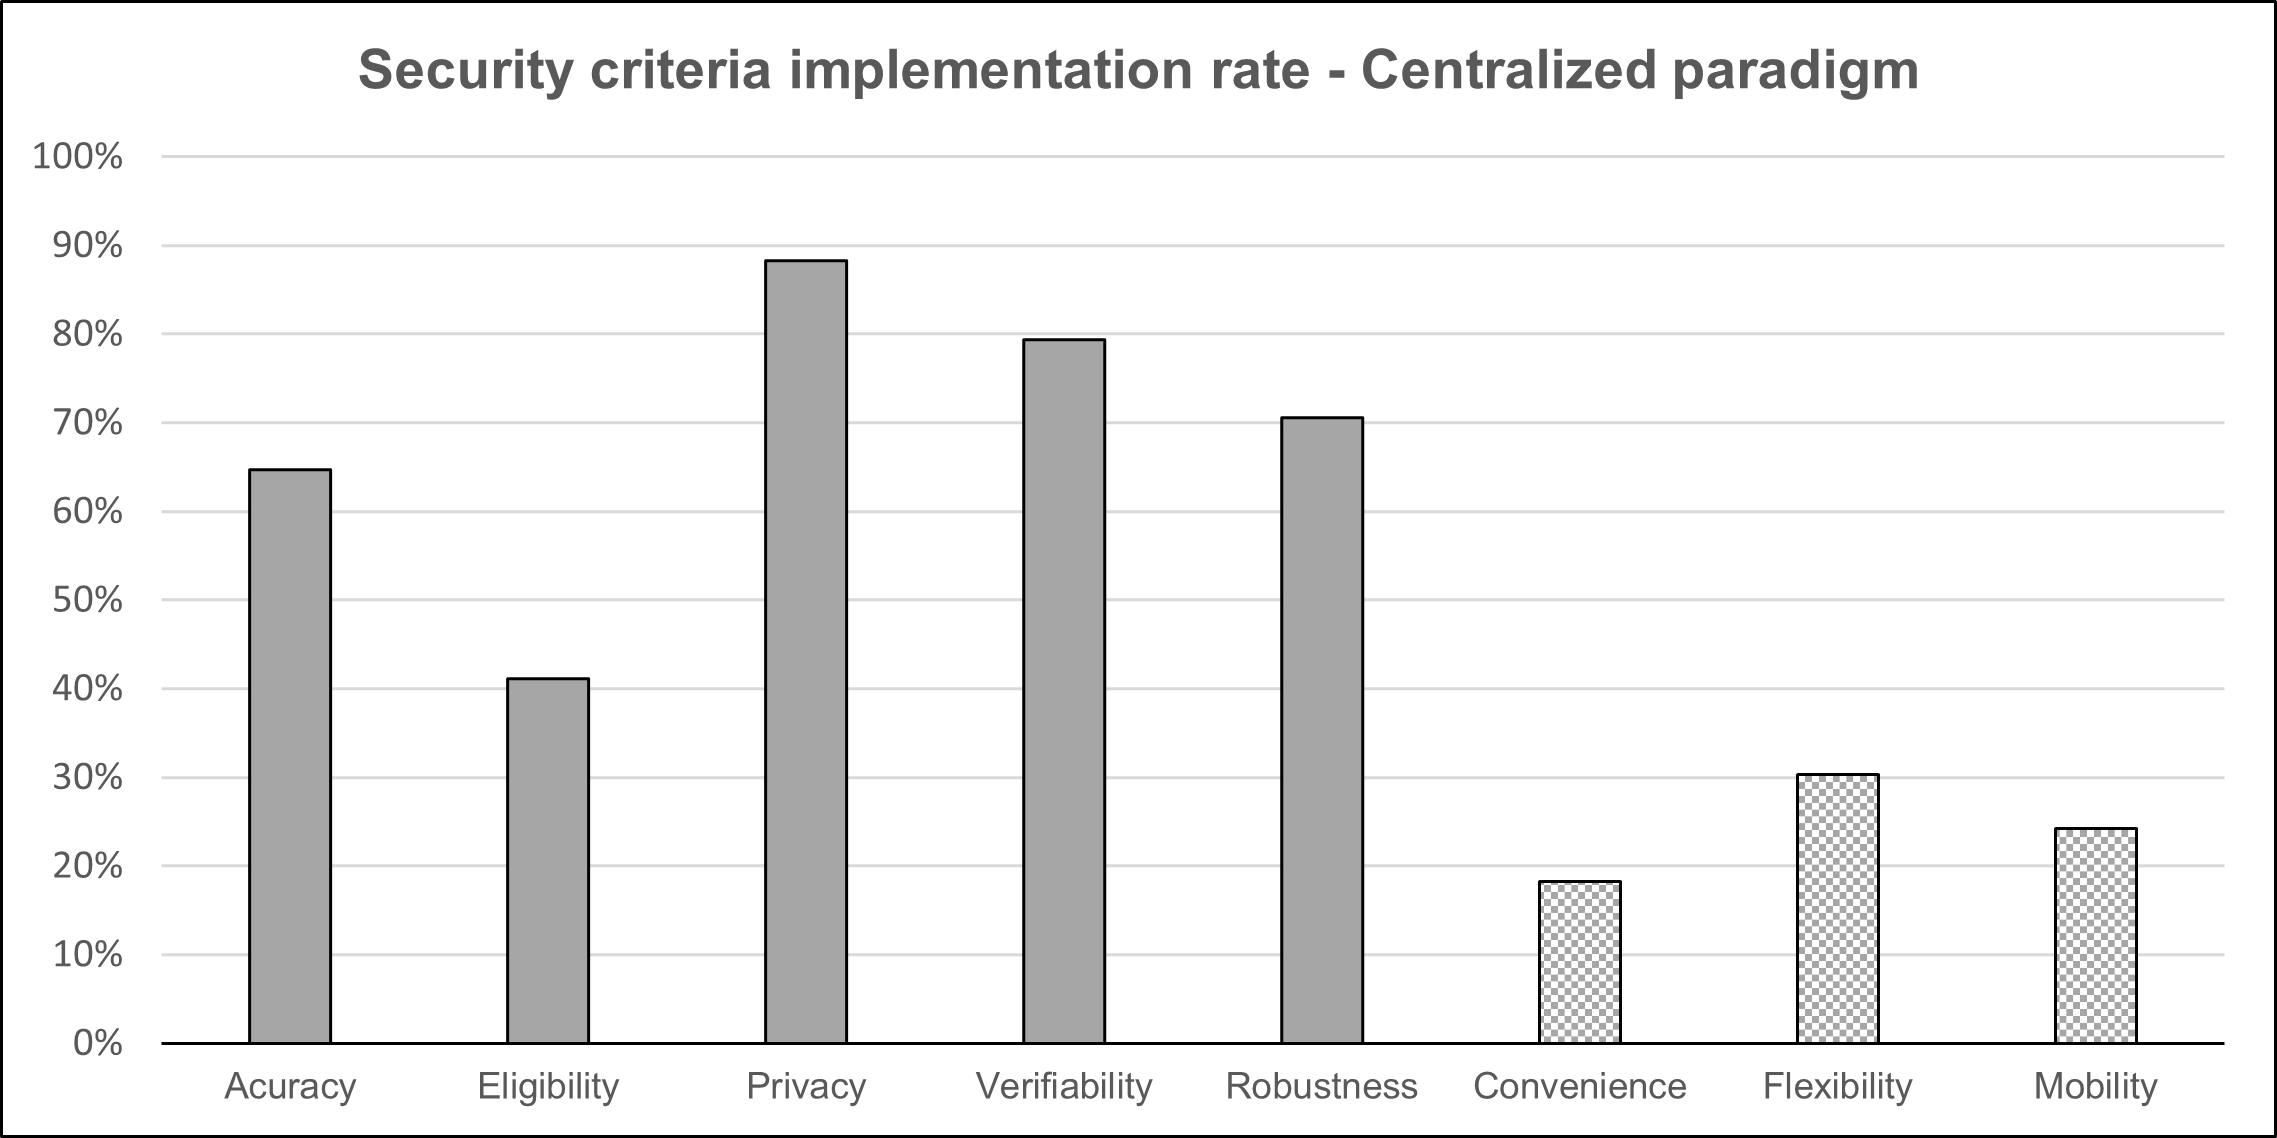
\includegraphics[width=\columnwidth]{Images/almei4.png}
        \caption{Statistical analysis of implementation rate.}
        \label{fig:implementation-rate-centralized}
    \end{figure}
    
    \subsubsection{Real-World Implementations of Centralised e-Voting Systems}
    \label{real-world-centralized}
    This section details a series of cases in which voting exercises with binding consequences were executed with, or aided with, electronic voting systems based on the centralised architectural paradigm. The main goal of these experiments was to determine the viability of the tool, security problems, public acceptability, etc.
    
    \paragraph{E-Voting Projects in Switzerland}
    As a means to determine the impact of increased availability on voter turnout, election costs, and potential security risks, the Swiss government established a series of e-voting trials centred around national referendums between 2004 and 2005.
    \par
    The system was unable to exchange data between cantons, the semi-autonomous regions in which Switzerland is divided, but it was nonetheless successful in anonymizing the votes and decoupling sensible voter information from the vote itself \cite{Binder2019}.
    \par
    The voting system was tested before deployment by a team of independent experts, with every identified flaw corrected before attempting the real exercise. The Swiss government successfully ran five independent trials in three cantons, all in national referendums. The first trial occurred in the Geneva canton in 2004. This exercise resulted in the lowest voter turnout percentage of all the online exercises, but the system was still able to attract 21.8\% of all eligible voters. The last of these trials happened in the Neuenburg canton, and this one recorded votes from 68\% of all eligible voters, indicating its acceptance by the population. Switzerland had among the highest levels of Internet penetration in Europe at the time, which may have contributed to the success of the online voting alternative \cite{Braun2006}.
    
    \paragraph{e-Voting in French Elections}
    The French government used the elections for the Lower Chambers of the Parliament in 2012 to trial an e-voting platform made available for expatriate voting. The French constitution had to be amended in order to address the legality of the new voting mechanism.
    \par
    French elections operate in rounds, and a successful identification in an earlier round carried on to the subsequent ones. All political parties involved in the election appointed observers, which joined a panel of supervisors with relevant governmental positions to observe the election process. The team of supervisors guaranteed that the vote count before the exercise's start was zero and that the final tally was consistent with the combined number of online and traditional voters.
    \par
    To test the system, a large-scale exercise with 15,000 volunteers was organized. During it, cybersecurity attacks were carried out on purpose by the National Agency for Security of Information Systems (ANSSI) to evaluate its response to outside attacks. Though the results were not published for security reasons, apart from problems derived from software compatibilities between the system and the voter's own systems, as well as problems with the identification process, the test was considered a success, and the e-voting system was approved for use in future elections \cite{Pinault2012}.
	
    \paragraph{Internet Voting in Canada}
    The first Canadian trials with Internet voting happened as far back as 2003, during the leadership elections for the Canadian New Democratic Party (NDP). The measure was successful and replicated in other cities and municipalities. In 2011, a national survey showed that 85\% of the country's population is favourable to an electronic alternative to complement the existing paper ballot system.
    \par
    There is scant information about the actual architectural implementation of these systems, with emphasis on the plural. Over the years, Canadians did trials with ever-changing systems, either due to security patches or simply updated once newer, faster hardware was made available. But considering the era in which these trials happened, it is safe to assume that they were conceived following a centralised, server-client architecture \cite{Goodman2014}.
    
    \paragraph{The Estonian I-voting System}
    \label{estonia_i_voting}
    Estonia was not the first to try remote e-voting systems, but it was the first country in the world to do so at a national level with binding consequences. The \textit{I-voting} system has been used widely in the country since 2005. That, alongside a developed telecommunications infrastructure, pushed 30\% of the eligible voters in the country to adopt the online alternative.
    \par
    The Estonian system uses a method that emulates the double-envelope system used in traditional voting. Voters can authenticate themselves using their national-issued ID card, which itself already possesses cryptographic capabilities on its own that can be used to both authenticate and protect ballot data, or a 2-factor authentication method that uses SIM card-based authentication.
    \par
    The \textit{I-voting} system was the first to use multiple vote casting as a measure to protect voters against coercive behaviour: the system allows multiple ballots to be cast by a single voter, but only the last one is counted. This allows voters to replace ballots cast under external coercive influence or if they simply changed their minds. But a physical vote always supersedes any online ones \cite{Heiberg2015}.
    \par
    Independent analysis revealed that the Estonian system was actually mired in security problems. System integrity was implemented by a series of protocols that were heavily dependent on human interaction, when these could have been automated with additional effort. When human errors eventually happened, these resulted in system errors and attacks. Since the complete source code was never published, it was impossible to guarantee the integrity of the tabulated results, which in itself is a significant lack of transparency.
    \par
    Because it is cheaper and simpler to maintain an online system than a traditional one, online voting in Estonia remains available for a longer period than the paper alternative. As an example, the October 2013 elections had a 7-day window for online voting. The outcome of this approach is mixed: on the one hand, the increased voting window allows voters more flexibility, giving them more time to make or change a decision. But on the other hand, keeping an unsecured system online for longer periods of time only increased the chances of success from attackers, especially for time-dependent attacks \cite{Madise2006}.
    \par
    The security problems with the Estonian e-voting system were thoroughly detailed in \cite{Finkenauer2014}. The conclusion was that the system was planned poorly from an architectural perspective.
    
    \paragraph{The Norwegian E-vote Project}
    Per request of the Norwegian government, a team of international experts from the International Foundation for Electoral Systems (IFES) independently oversaw extensive tests of the Norwegian \textit{E-vote} online solutions in a series of less consequential elections, such as local referendums and youth council elections.
    \par
    The Norwegian approach is similar to the Estonian one: both systems take advantage of a national-wide, government-issued identification system with built-in cryptographic capabilities. The Norwegian MiniID system is a 2-factor authentication system enabled and available by default to all Norwegian citizens, requiring only an active mobile phone number to receive a one-time password to register. The \textit{E-vote} system also addresses voter coercion with a multiple vote casting feature, similar to the Estonian case \cite{Barrat2012}.
    \par
    Regarding the difficulties and problems, this solution was also plagued by the same problems already identified in a similar, centralised model, namely, software incompatibilities between the centralised interface and the multitude of options with which a voter might interact with the system. To mitigate them as much as possible, the \textit{E-vote} system was developed to be accessed as a public web application. Developers had to take into account all the potential operating systems and Internet browsers at development time, which increased the system complexity without any gains in security, transparency, and/or scalability \cite{Binder2019}.
    
    \paragraph{The New South Wales iVote System}
    The Australian region of New South Wales introduced its centralised e-voting system in March 2015. The development and deployment of the \textit{iVote} system were supervised by the New South Wales Electoral Commission (NSWEC). Results were positive in terms of popular acceptance, with 5\% of all votes being cast with the tool. The percentage itself is not significant in the overall exercise, but taking into account the population density of the region (which includes Sydney, one of Australia's largest cities), that percentage amounts to over 280,000 votes, which is more than any of the other exercises considered thus far.
    \par
    The \textit{iVote} system was also subjected to an unscheduled security review by an independent team of experts, which identified several flaws that stem from the centralised nature of the application, namely:
    \begin{itemize}
        \item {Susceptibility to \textit{downgrade-to-export} attacks, where the system can be "tricked" to swap a high-security communication protocol for a low-security one that can then be attacked more easily.}
        \item {Use of the breakable Transport Layer Security (TLS) protocol when the Secure Sockets Layer (SSL) protocol was already available at the time.}
        \item {Code permeability, which allowed for injections of malicious code through the voter's browser}
    \end{itemize}
    Though these problems were identified before the real exercise, their solution, through code patching, occurred during the voting period, which created a time window in which the system could have been attacked with the security flaws still active. 3177 votes decided one of the races in that election. Further calculations revealed that the vulnerability window could have affected around 66,000 votes, which could have easily produced erroneous results in the election.
    \par
    Though it seemed unlikely that the \textit{iVote} system had been perverted during that exercise, the damage to the perception of trust by these tools could have been disastrous if such an attack had taken place. Besides these problems, the system behaved as intended, and the population was satisfied with its performance \cite{Halderman2015}.

    \subsubsection{Conclusion}
    This analysis is able to elucidate regarding research question \textbf{RQB2} in section \ref{general-research-questions}, namely, how the cryptographic protocols and methods identified during the initial analysis had translated to real-world applications. And the answer is that they do not appear to. Despite all the work and ideas that originated the cryptographic methods, their effect on real-world applications seems marginal at best.
    \par
    This analysis was somewhat superficial due to the proprietary nature of the solutions presented. Most of the publications reviewed were only suited to serve small-based voting exercises, but every real-world solution considered, even if not available to all eligible voters, processed a number of votes far beyond a number that could qualify these exercises as "small". This by itself, alongside the unsolved inherent limitations associated with a centralised model, excludes the utilisation methods hard to scale up, such as \textit{Blind Signatures} or \textit{Cryptographic Proofs}. The absence of mentions of these methods in either the documentation available or any of the independent reports produced supports this hypothesis.
    \par
    It appears that the involved governments ordered software solutions for private companies, and these devised solutions based on existing and tried approaches from other industries, such as e-commerce and e-banking applications, and modelled the voting process around them. Given that all these exercises were moderately successful, even with security flaws identified, the strategy employed is not completely unfit but does ignore the academic research. The authentication methods employed are a testament to this assumption: 2-Factor Authentication schemes are becoming the norm whenever sensitive information, such as account numbers and balance, or personal information, is in play.
    \par
    The real-world implementations analysed are pertinent examples of how important an alternative to traditional voting is. Though they do seem to ignore most academic research on the subject in the last few years, they still represent an important starting point for a transition between theoretical ideas and practical implementations.
    \twocolumn
\end{document}